\chapter{Introduction}
Orthogonal codes are a widely adopted technology in various fields, including telecommunications and wireless communications. One of the most promising areas for the application of orthogonal codes is in underwater acoustic localization. Acoustic signals are widely used for underwater communication due to their ability to propagate well in water. However, the harsh underwater environment poses many challenges for accurate localization, such as multipath propagation and noise.

This research project proposes the use of pseudorandom binary codes for underwater acoustic localization. The codes are processed and then transmitted via hydrophones, and multiple sending anchors are used to increase the accuracy of the localization. Time-difference-of-arrival (TDOA) correlation techniques are employed to estimate the position of a target in 3D space using the signals received by the anchors. The use of orthogonal codes can improve the robustness of the localization system against noise and multipath propagation. The aim is to examine the performance of various code types and design strategies to select the optimal code. This research endeavors to enhance the precision and dependability of underwater localization systems through the utilization of orthogonal codes, with the ultimate goal of facilitating a plethora of applications, including but not limited to oceanographic studies and undersea navigation. 

One specific example of this application would be the use in the BlueROV2 \ref{fig:bluerov}, a remotely operated underwater vehicle, which would greatly benefit from  this method of localization.

\begin{figure}[h]
	\centering
	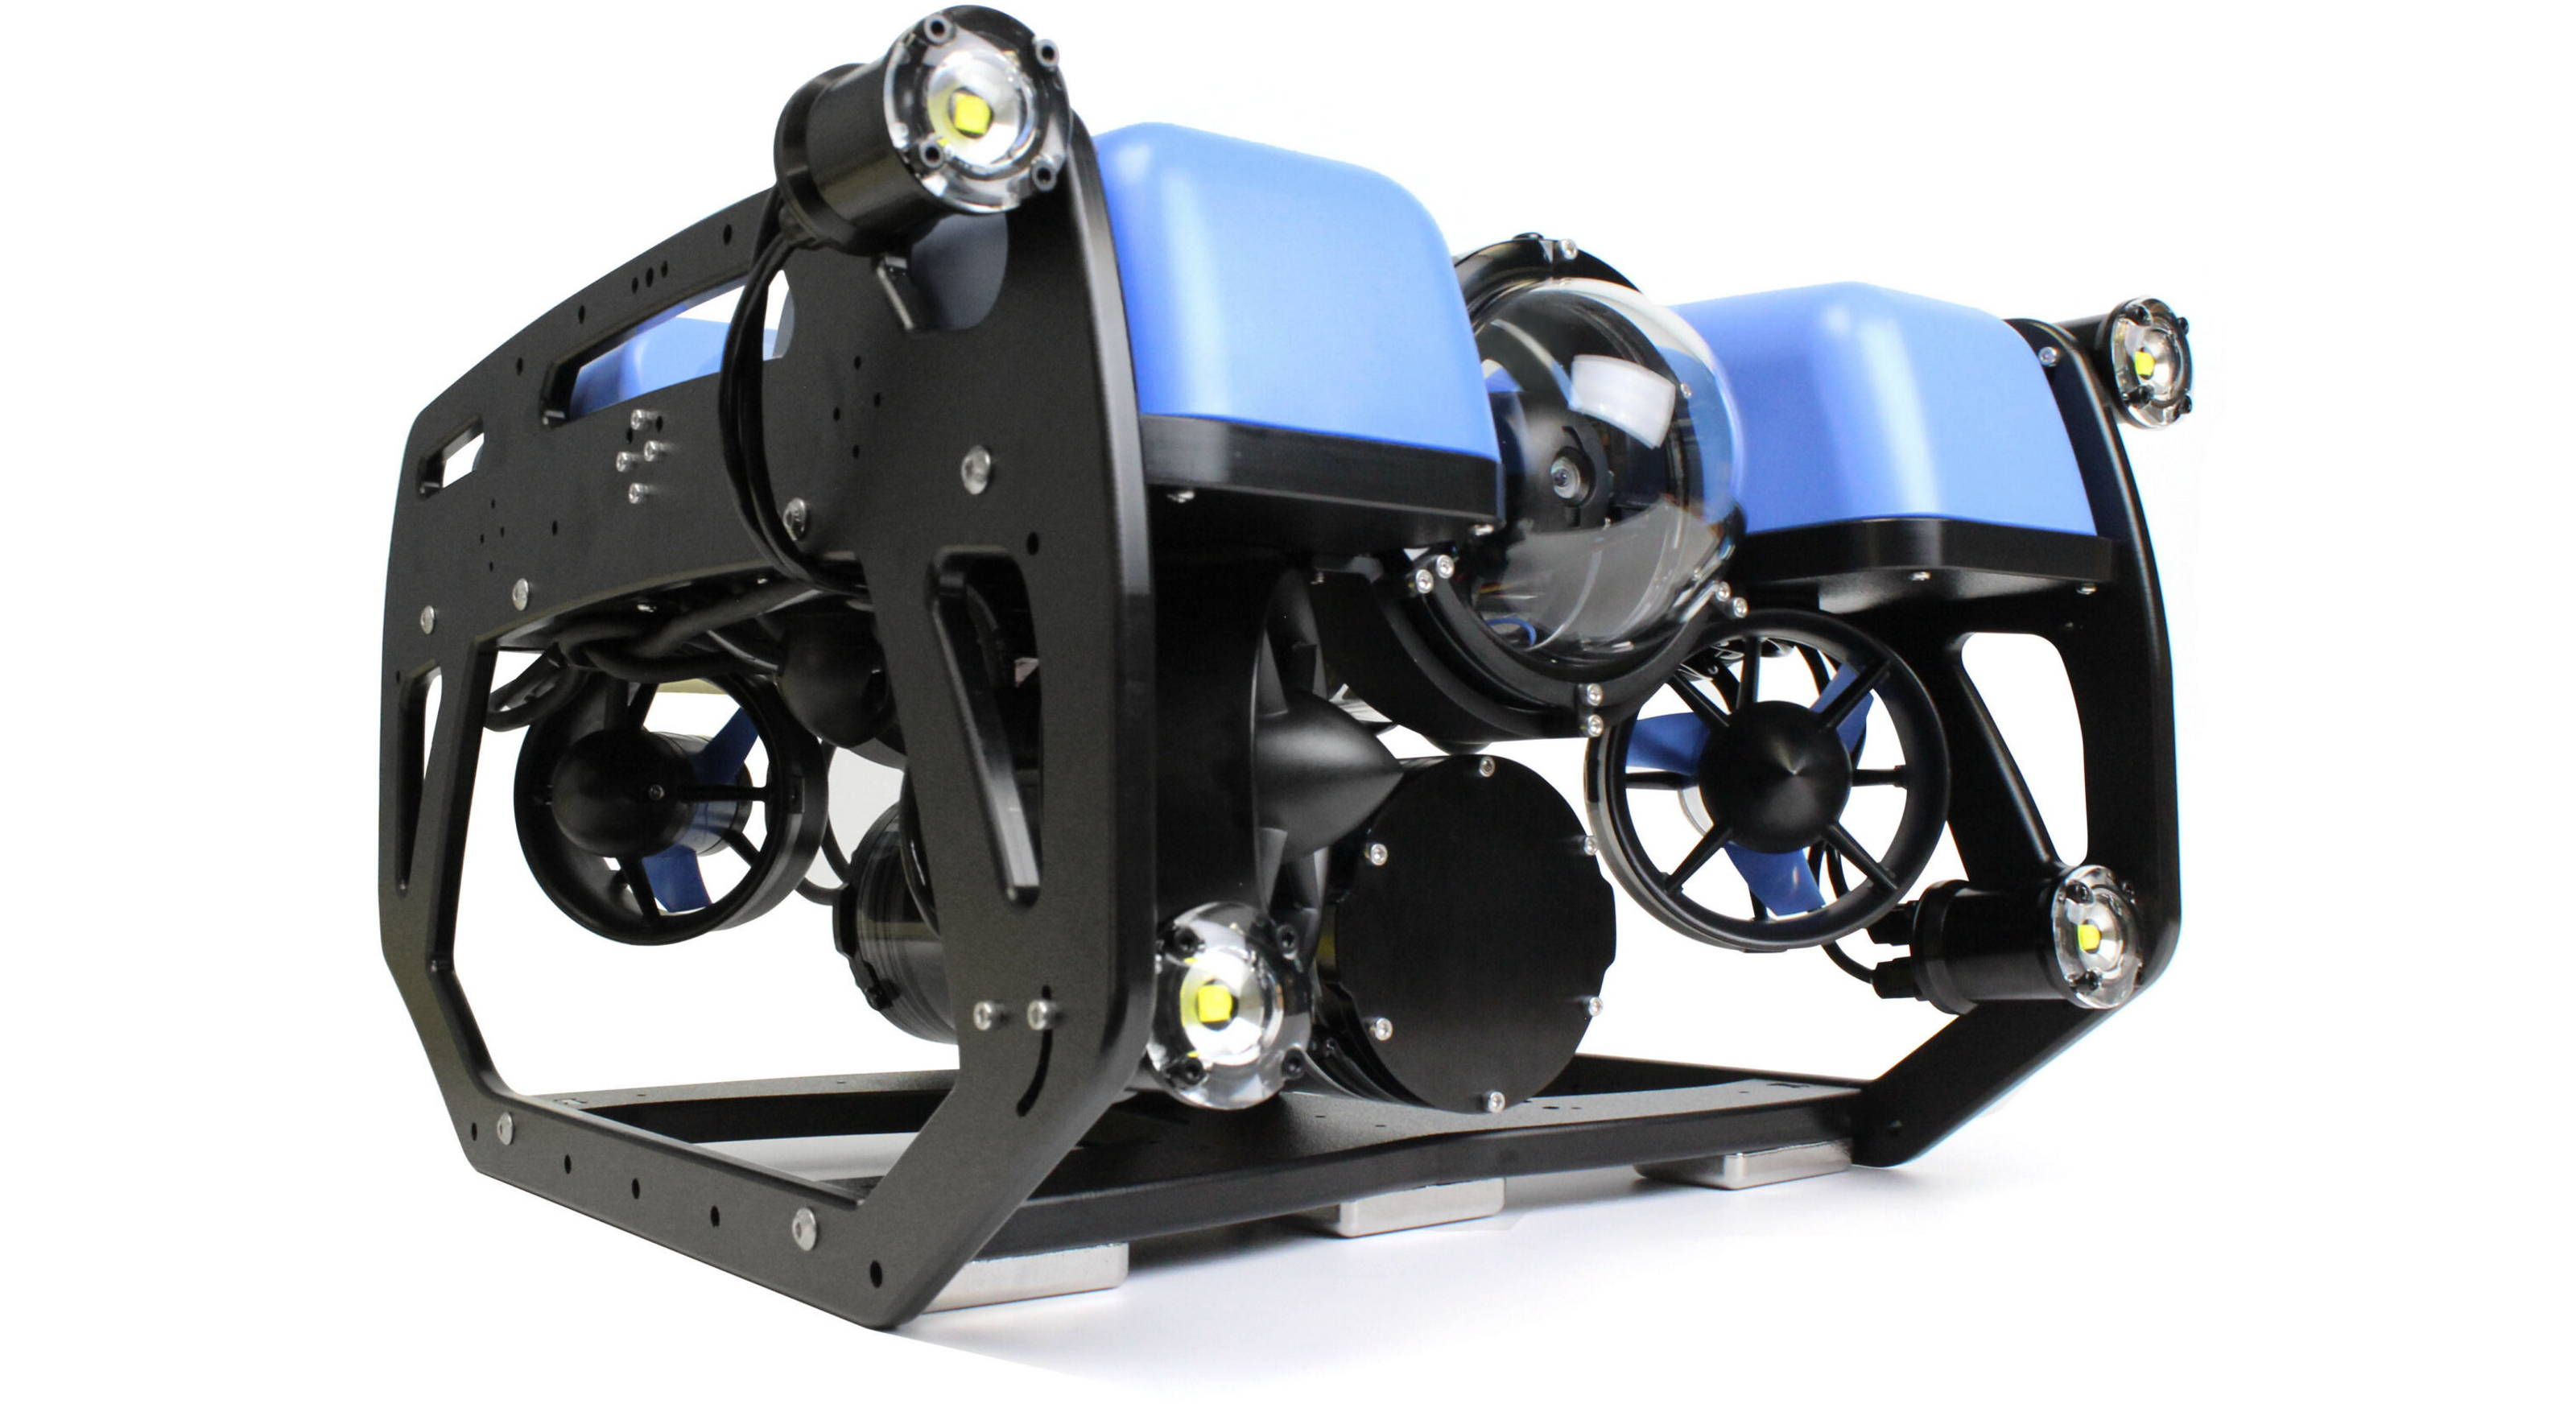
\includegraphics[width=5.5cm]{images/bluerov}
	
	\caption{BlueROV2 from Blue Robotics Inc}
	\label{fig:bluerov}
\end{figure}
\section{Motivation} 
The principle of Time Difference of Arrival (TDOA) has been widely adopted in GPS applications for localizing small devices or mobile vehicles. However, this principle has yet to be fully explored for its potential in underwater localization. Unlike GPS, which utilizes electromagnetic waves, acoustic communication is required for underwater localization due to the high damping of electromagnetic waves underwater. This can be achieved through the use of hydrophones, piezoelectric transducers that are capable of receiving and sending underwater acoustic signals.

The current underwater localization systems rely on the underwater vehicle transmitting signals to anchored beacons. However, this project aims to reverse this approach, allowing multiple underwater vehicles to localize themselves with the help of signals transmitted by the beacons. In theory, multiple underwater vehicles should be able to simultaneously localize themselves without interference, making this project a valuable contribution to the development of more accurate and reliable underwater localization systems.
\section{Setup and objectives}
The study will commence with an examination of orthogonal codes, signal processing and modulation techniques. This will include a review of cross-correlation and auto-correlation concepts to ensure a solid understanding of the fundamental principles. Subsequently, the focus will shift towards understanding underwater communication and the transmission of acoustic signals through piezoelectric transducers.

Based on the knowledge gained, the study will move forward with the implementation of a self-localization system in 3D space using four anchors, which will be based on orthogonal codes and a  appropriate peak detection algorithm. The initial phase of development will take place in MATLAB, followed by a switch to Python. The only exception will be the use of a benchmark tool, which will remain in MATLAB.
Upon completion of the implementation, the performance of the algorithms will be evaluated in various scenarios. If the results are found to be satisfactory, the evaluation will be extended with a simplified field test in real-world conditions. 

In summary, the research project aims to uncover valuable insights into using orthogonal codes for self-localization in underwater environments, and to implement a localization system. The project will conclude with a comprehensive evaluation and comparison of the implemented algorithm.